%!TeX root=MemoriaTFG.tex

\chapter{Gràfiques addicionals dels experiments}
\label{ann:grafiques}

Aquest annex recull les figures generades pels notebooks d'anàlisi que no han
tingut cabuda al cos principal de la memòria per raons d'espai o perquè
aporten detall complementari, no el resultat central de cada fase.

% ---------------------------------------------------------------
\section{Bloc 1: Comparació inicial i curriculum learning}
% ---------------------------------------------------------------

\subsection{Fase 1: Comparació d'algorismes}


\begin{figure}[H]
  \centering
  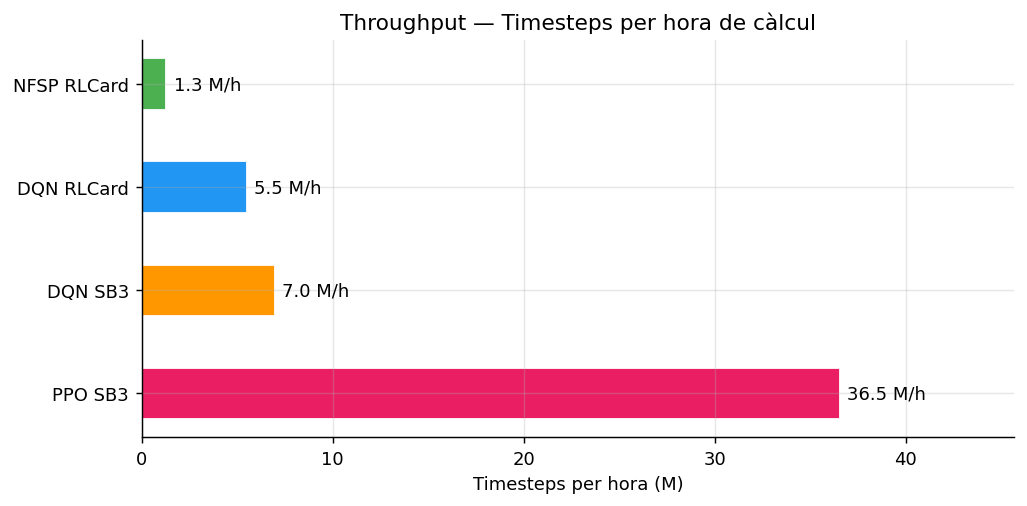
\includegraphics[width=0.7\textwidth]{figures/fase1/cell15.png}
  \caption[Velocitat d'entrenament dels quatre algorismes (M passos/hora).]{Velocitat d'entrenament en milions de passos per hora de càlcul.
           \ac{PPO}-\ac{SB3} és 28~vegades més ràpid que \ac{NFSP}-RLCard gràcies
           al paral·lelisme de múltiples entorns.}
  \label{fig:ann-fase1-throughput}
\end{figure}

\subsection{Fase 2: Curriculum learning}

\begin{figure}[H]
  \centering
  
\includegraphics[width=\textwidth]{figures/fase2/cell06.png}
  \caption[Grup de control de la Fase~2 (24M passos en partides, sense currículum).]{Grup de control de la Fase~2: entrenament directament sobre partides senceres
           durant 24M passos, sense passar per mans. \ac{DQN}-\ac{SB3} és l'únic que
           supera el 50\% contra l'agent basat en regles; els altres tres no superen el 25\%.}
  \label{fig:ann-fase2-control}
\end{figure}


\begin{figure}[H]
  \centering
  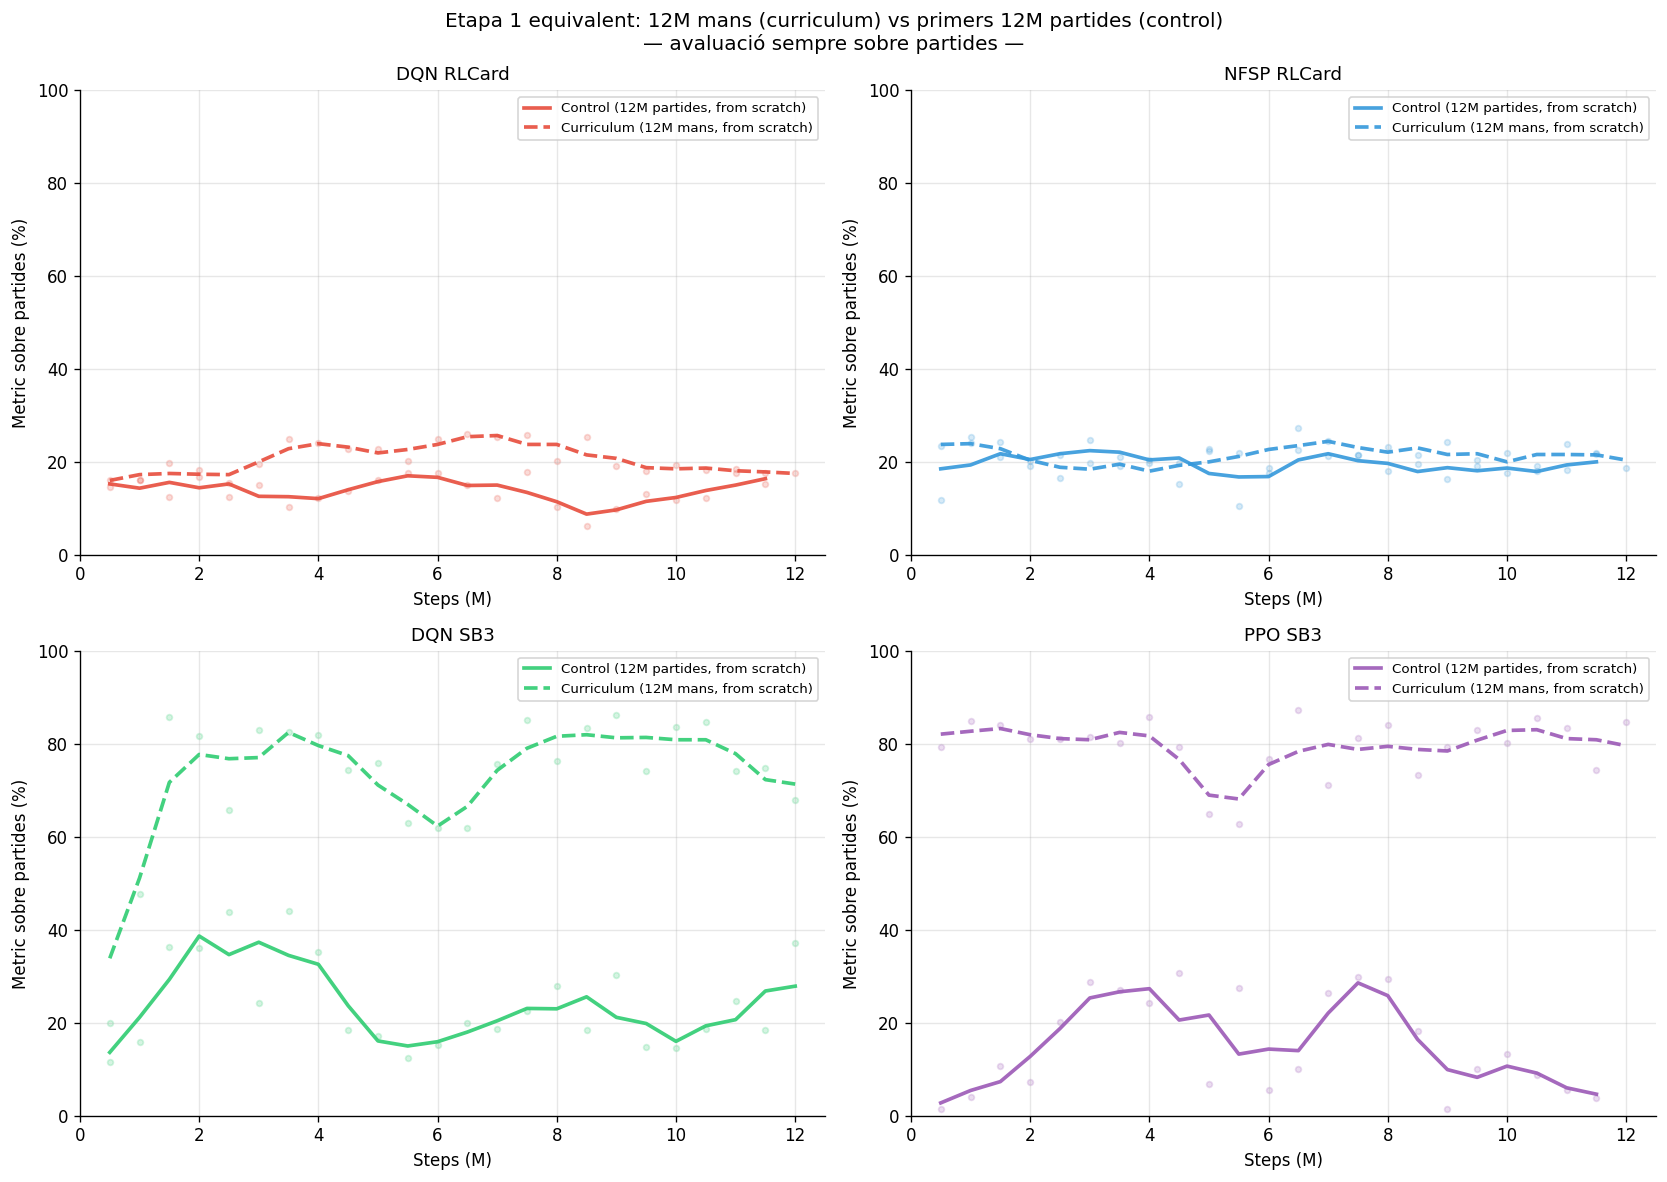
\includegraphics[width=\textwidth]{figures/fase2/cell14.png}
  \caption[Comparació directa mans vs partides a pressupost equivalent (Fase~2).]{Comparació de l'etapa 1 equivalent: 12M passos sobre mans (currículum)
           contra els primers 12M passos directament sobre partides (control). En
           els agents \ac{SB3}, les mans eleven la mètrica molt per sobre del control;
           en els de RLCard la diferència és mínima.}
  \label{fig:ann-fase2-etapa1}
\end{figure}

\begin{figure}[H]
  \centering
  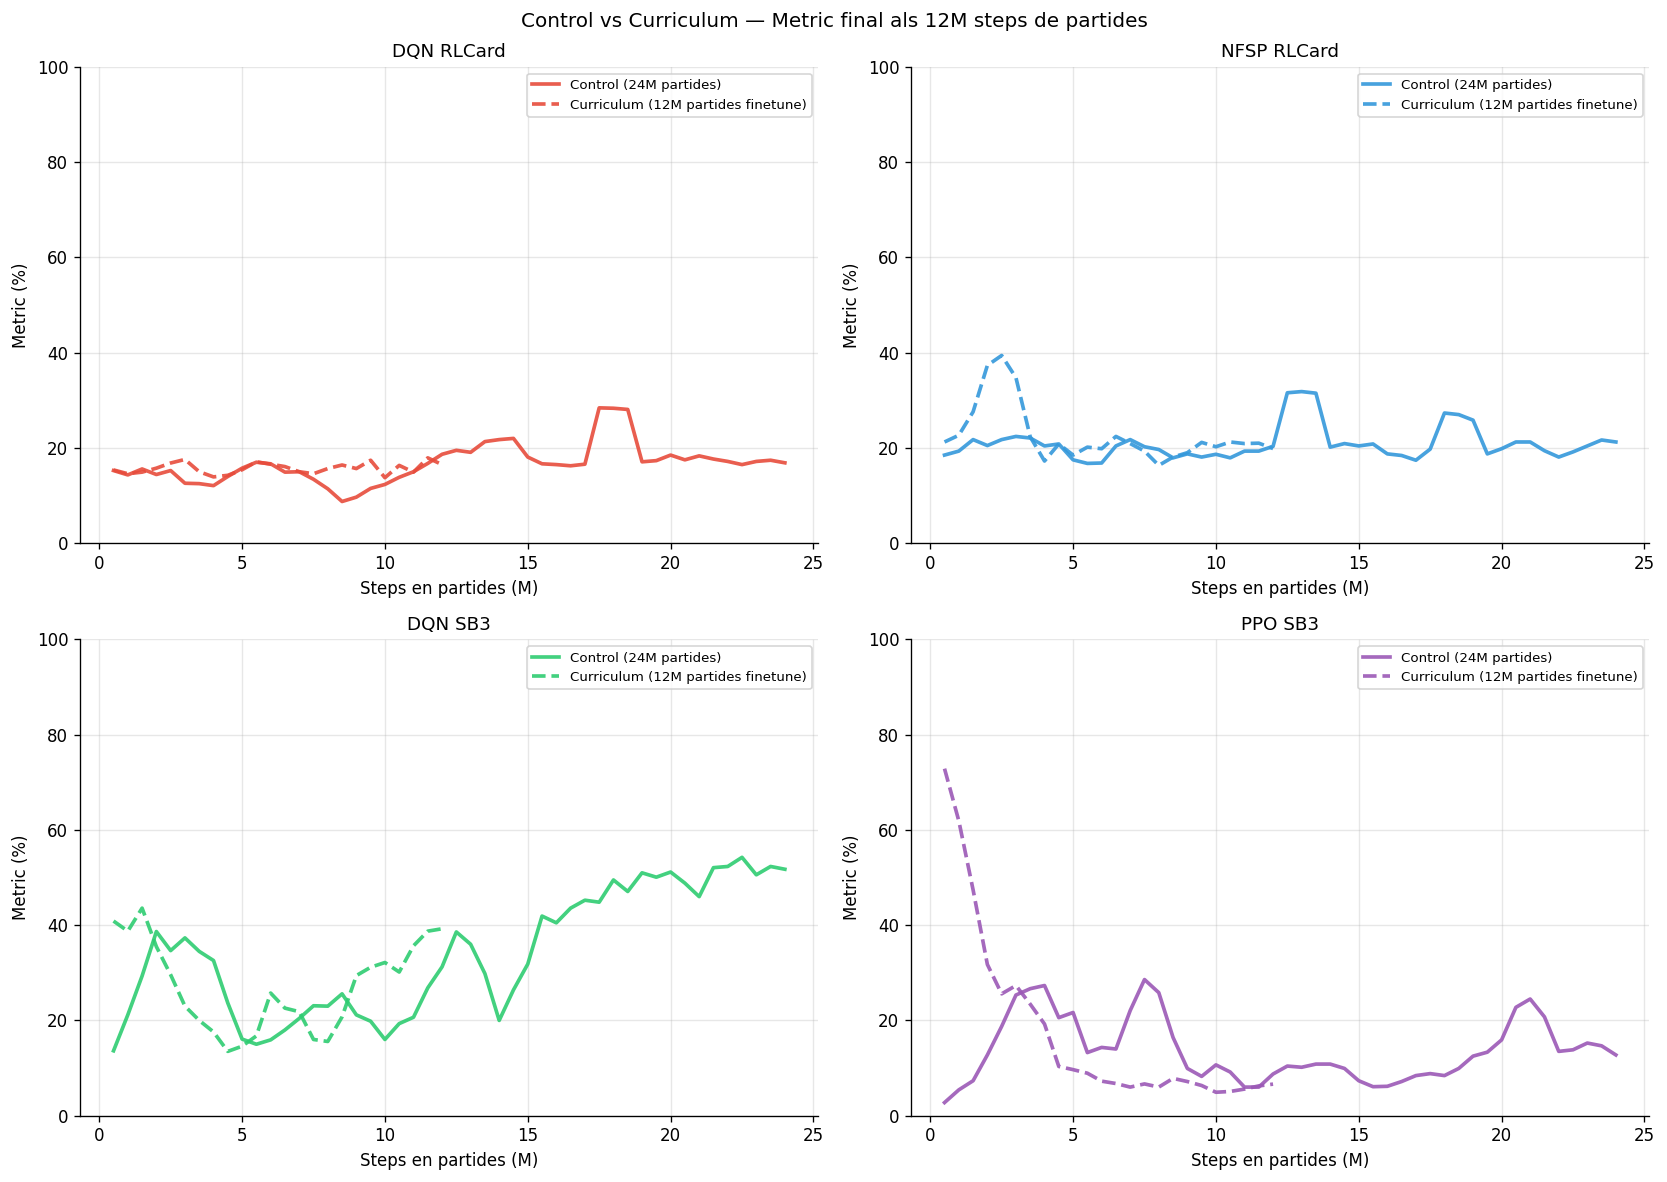
\includegraphics[width=\textwidth]{figures/fase2/cell12.png}
  \caption[Control vs currículum als 12M passos de partides (Fase~2).]{Control vs currículum al final de l'etapa de partides (12M passos de
           \emph{finetune}). El currículum (línia discontínua) degrada els agents
           \ac{SB3} per sota del seu control, evidenciant l'oblit catastròfic.}
  \label{fig:ann-fase2-ctrl-vs-curr}
\end{figure}

\begin{figure}[H]
  \centering
  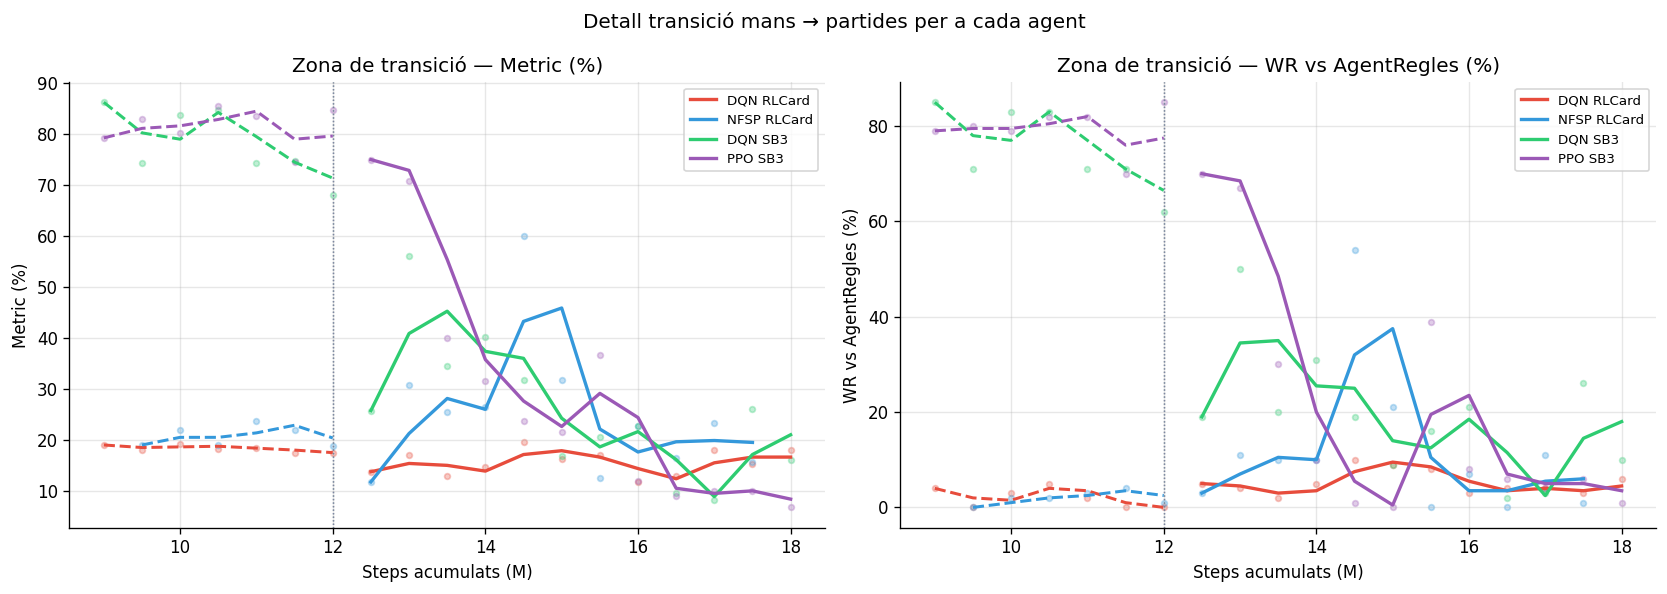
\includegraphics[width=\textwidth]{figures/fase2/cell16.png}
  \caption[Zona de transició mans~$\rightarrow$~partides (Fase~2).]{Detall de la zona de transició mans~$\rightarrow$~partides. La línia
           puntejada vertical marca el canvi de protocol (12M passos). \ac{PPO}-\ac{SB3}
           mostra la caiguda més dràstica: de 80\% a menys del 10\% en pocs
           checkpoints.}
  \label{fig:ann-fase2-transicio}
\end{figure}

% ---------------------------------------------------------------
\section{Bloc 2: Representació de l'estat i memòria}
% ---------------------------------------------------------------

\subsection{Fases 3 i 3.5: Extractor de característiques}

\begin{figure}[H]
  \centering
  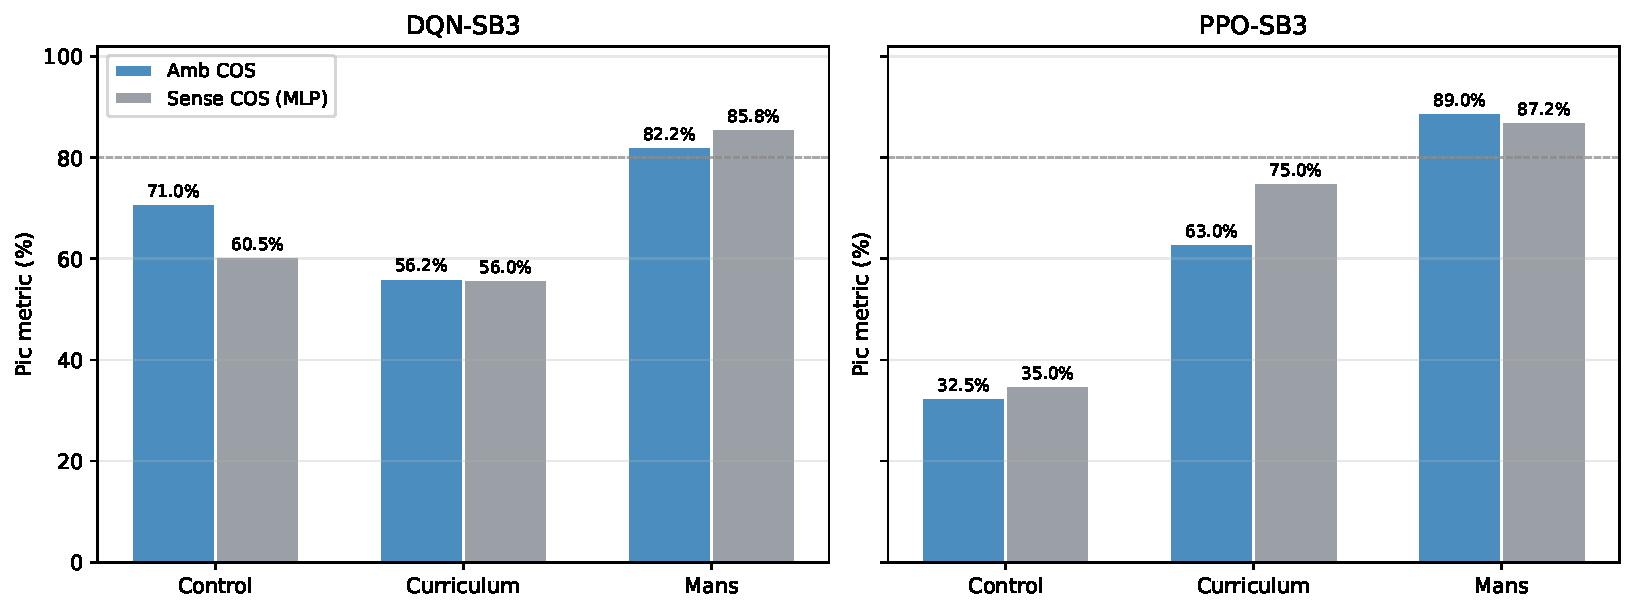
\includegraphics[width=\textwidth]{figures/fase3/fase3_cos_vs_mlp.pdf}
  \caption[Pic de mètrica COS vs MLP per protocol i agent (Fase~3).]{Pic de win-rate ponderat per als protocols de control, currículum i mans,
           comparant l'extractor \emph{CosMultiInput} (blau) contra el \ac{MLP} pla
           (gris). El COS no supera sistemàticament el \ac{MLP}: la diferència és
           rellevant només al control de \ac{DQN}-\ac{SB3}.}
  \label{fig:ann-fase3-cos-mlp}
\end{figure}

\subsection{Fase 4: Memòria recurrent i pool d'oponents}

\begin{figure}[H]
  \centering
  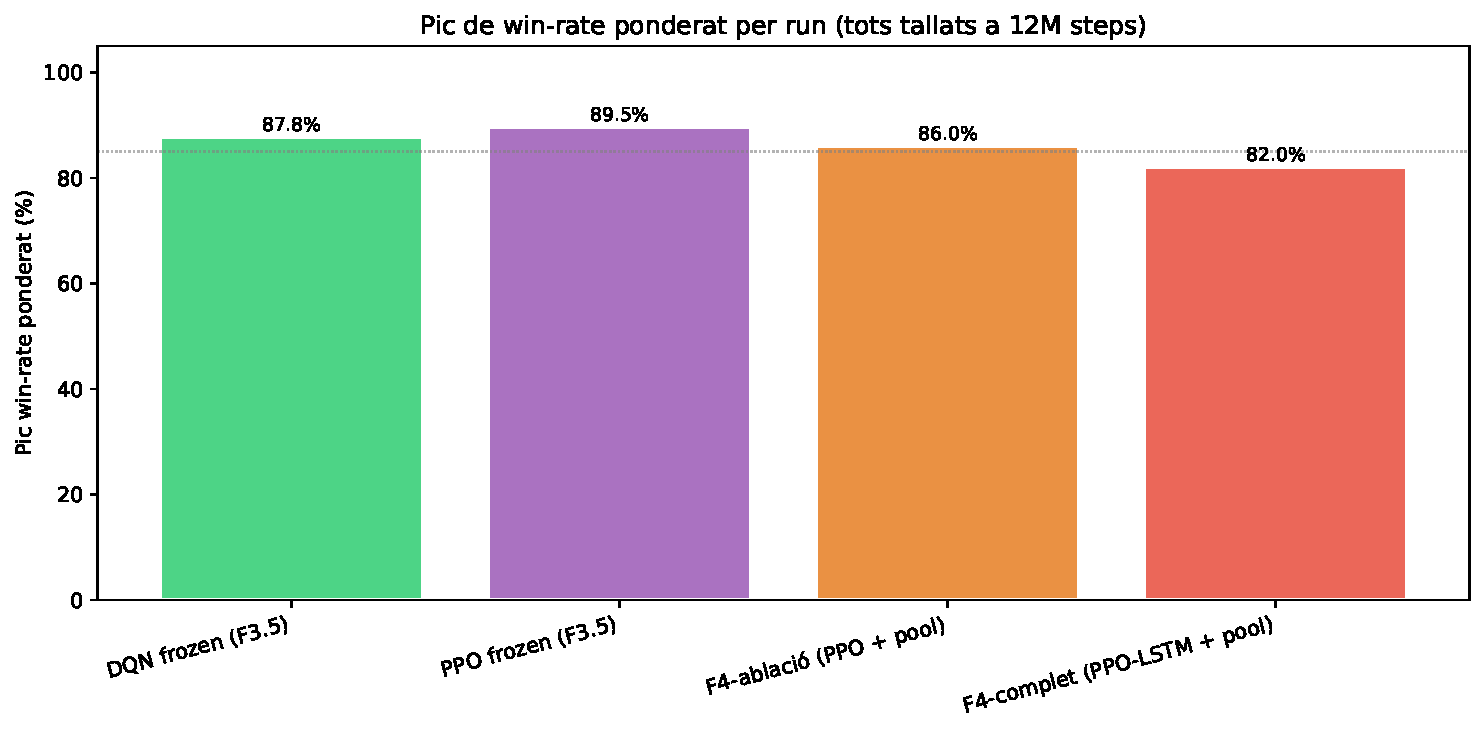
\includegraphics[width=0.85\textwidth]{figures/fase4/fase4_barplot.pdf}
  \caption[Pic de win-rate ponderat per variant de la Fase~4 (12M passos).]{Pic de win-rate ponderat per als quatre entrenaments de la Fase~4,
           tots tallats a 12M passos. \ac{PPO} frozen (F3.5) assoleix el màxim
           (89{,}5\%), seguit de \ac{DQN} frozen (87{,}8\%). L'afegit de
           \ac{LSTM} (F4-complet) no millora el pic en aquest pressupost.}
  \label{fig:ann-fase4-barplot}
\end{figure}

% ---------------------------------------------------------------
\section{Bloc 3: selecció del model de desplegament (Checkpoint~3)}
% ---------------------------------------------------------------

\begin{figure}[H]
  \centering
  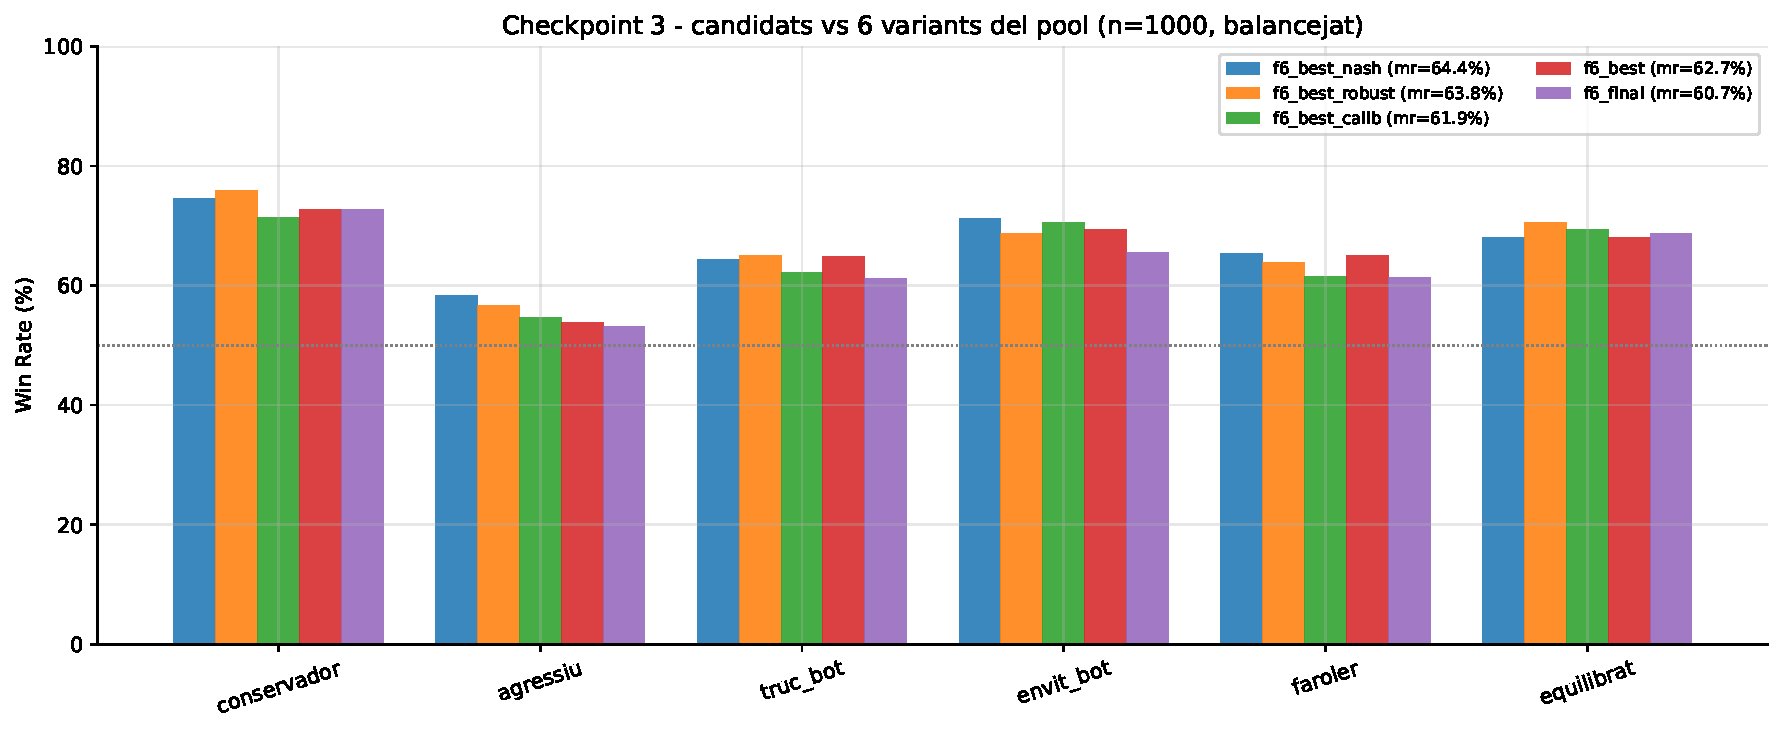
\includegraphics[width=\textwidth]{figures/checkpoint3/comparacio_candidats.pdf}
  \caption[Win-rate dels candidats del Checkpoint~3 vs les 6 variants del pool.]{Win-rate de cada candidat contra les sis variants del pool
           (1\,000~partides balancejades). \texttt{f6\_best\_nash} (blau) assoleix la
           \(\text{metric\_robust}\) més alta (64{,}4\%) i és el model seleccionat.}
  \label{fig:ann-cp3-candidats}
\end{figure}


\begin{figure}[H]
  \centering
  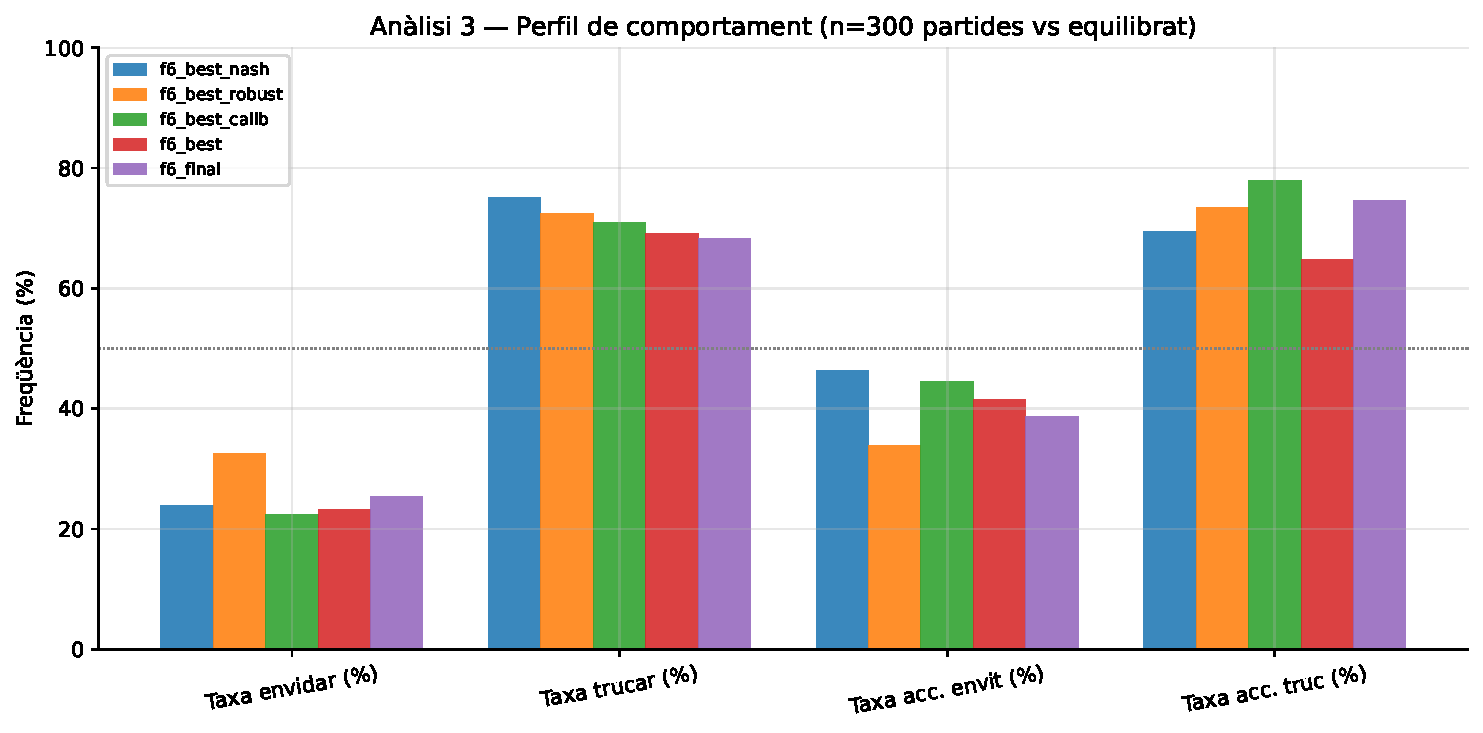
\includegraphics[width=\textwidth]{figures/checkpoint3/perfil_comportament.pdf}
  \caption[Perfil de comportament dels candidats del Checkpoint~3.]{Freqüències d'acció dels cinc candidats (300 partides vs agent
           equilibrat). \texttt{f6\_best\_nash} mostra la taxa d'envidar més baixa
           i la taxa d'acceptació del truc moderada, coherent amb una política
           de menor risc.}
  \label{fig:ann-cp3-perfil}
\end{figure}

\begin{figure}[H]
  \centering
  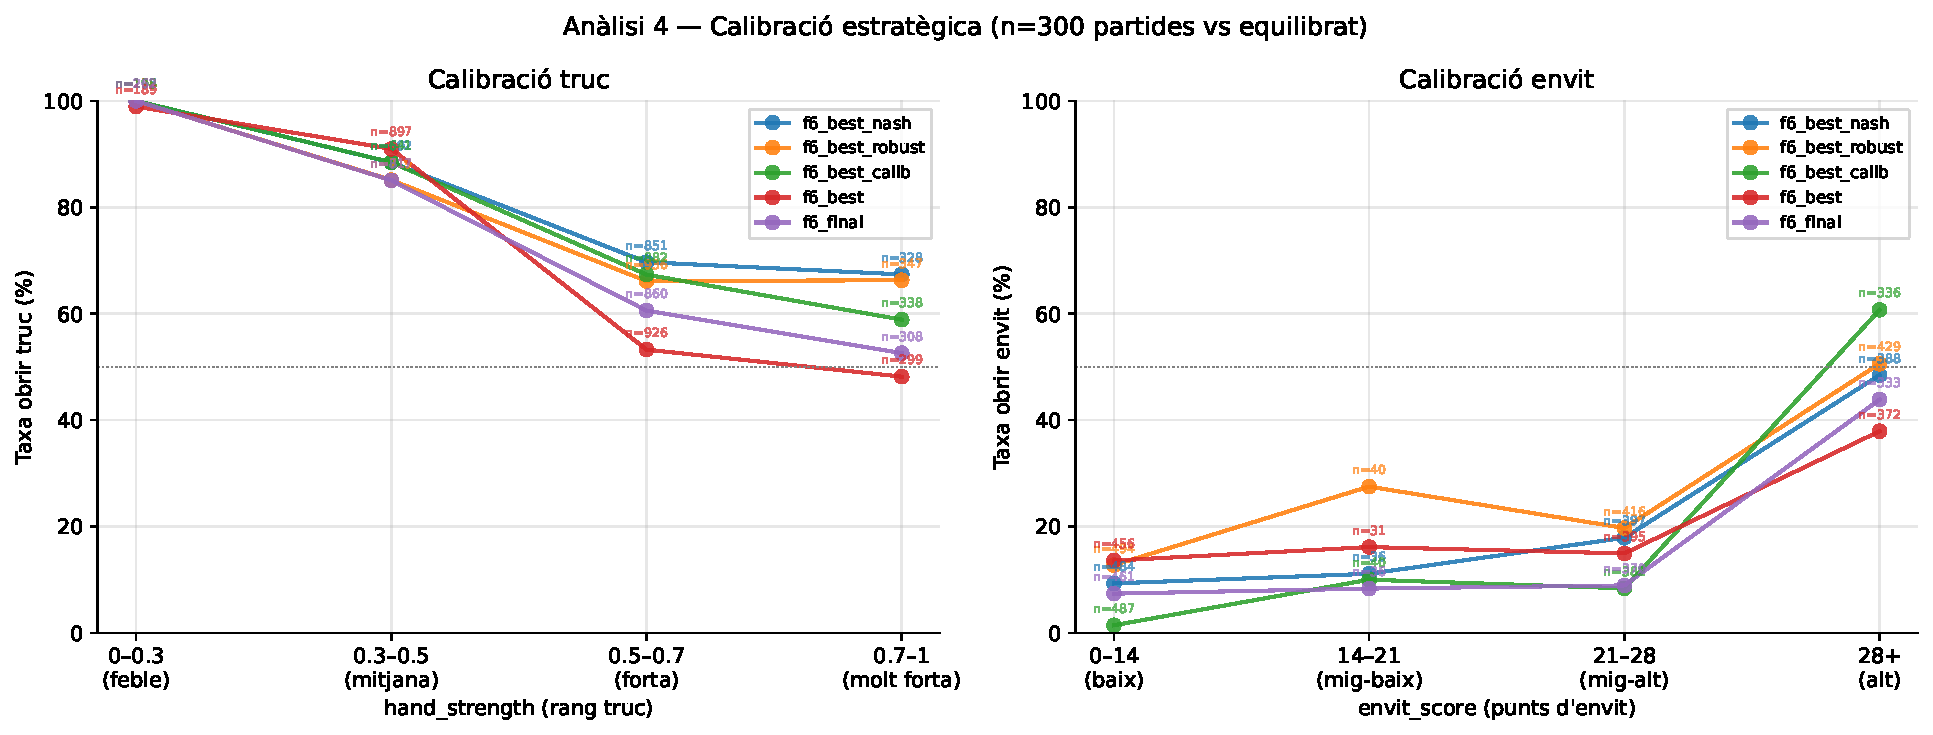
\includegraphics[width=\textwidth]{figures/checkpoint3/calibracio_estrategica.pdf}
  \caption[Calibració estratègica dels cinc candidats del Checkpoint~3.]{Taxa d'obrir truc per franja de força de mà (esquerra) i taxa d'obrir envit
           per puntuació d'envit (dreta) dels cinc candidats (300 partides vs agent
           equilibrat). Tots mostren el patró de farol al truc (decreixent amb la
           força) i una política d'envit creixent amb la puntuació; les diferències
           entre candidats són petites, cosa que confirma que la selecció es basa en
           el Nash gap i no en el comportament qualitatiu.}
  \label{fig:ann-cp3-calibracio}
\end{figure}

% ---------------------------------------------------------------
\section{Anàlisi del model final}
% ---------------------------------------------------------------

\begin{figure}[H]
  \centering
  \includegraphics[width=0.75\textwidth]{figures/resultats/rendiment_oponents.pdf}
  \caption[Win-rate del model desplegat per oponent (barres).]{Win-rate de \texttt{best\_nash} contra cada oponent (1\,000~partides
           per oponent). L'oponent agressiu és el més difícil (55\%); contra
           si mateix el resultat és del 50\%, consistent amb l'equilibri de Nash.}
  \label{fig:ann-res-rendiment-barres}
\end{figure}


\begin{figure}[H]
  \centering
  
\includegraphics[width=\textwidth]{figures/resultats/calibracio_estrategica.pdf}
  \caption[Calibració estratègica del model desplegat (heatmap).]{Heatmap de la probabilitat d'obrir truc (esquerra) i d'obrir envit (dreta)
           en funció conjunta de la força de mà i els punts d'envit, amb la
           mostra per cel·la. Complementa la figura~\ref{fig:ann-cp3-calibracio}
           mostrant la política del model final en dues dimensions simultàniament.}
  \label{fig:ann-res-calibracio}
\end{figure}

\begin{figure}[H]
  \centering
  \includegraphics[width=0.6\textwidth]{figures/resultats/estil_radar.pdf}
  \caption[Perfil d'estil emergent del model desplegat (diagrama de radar).]{Perfil d'estil emergent del model desplegat (vermell) comparat amb
           l'agent basat en regles equilibrat (blau) en cinc dimensions de context.
           El model mostra una agressió al truc superior i una propensió a l'envit
           inferior a la de l'agent de regles.}
  \label{fig:ann-res-radar}
\end{figure}
